\chapter{Differentially heated cavity}

The differentially heated cavity problem or buoyancy-driven cavity problem is a two dimensional problem based on free convection. It comprises a cavity with the vertical walls at different temperatures and adiabatic horizontal walls \cite{DeVahlDavis1983a, DeVahlDavis1983}. The difference of temperatures between the two vertical walls causes convection.

\begin{figure}[h]
	\centering
	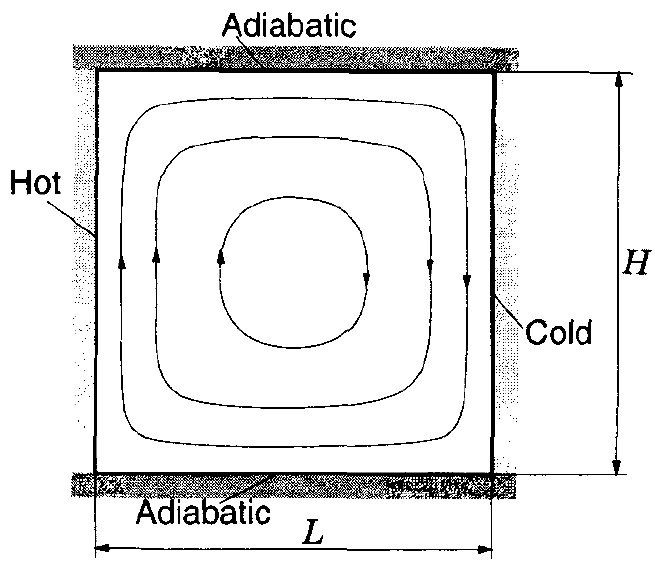
\includegraphics[scale=0.5]{Buoyancy/BuoyancyDriven}
	\caption[General scheme of the differentially heated problem]{General scheme of the differentially heated problem. Extracted from \cite{Ferziger2002}}
\end{figure}

\section{Natural convection}
The equations that are going to be discretized are the two-dimensional equations of mass, momentum and energy for a Newtonian fluid with constant properties. However, some approximations have to be done for the momentum equation:
\begin{equation}
\rho_{0}\frac{\partial\vec{v}}{\partial t}+\rho_{0}\left(\vec{v}\cdot\nabla\right)\vec{v}=-\nabla p+\mu\nabla^{2}\vec{v}+\rho\vec{g}
\end{equation}
As it can be seen, mass forces have been added to the momentum equation, because in natural convection gravity is not negligible. Another important remark is that the fluid is considered incompressible, but this approximation is not applied in the gravitational term, because it is this term that causes the flow. However, as a simplification, the Boussinesq approximation is applied \cite{Bergman2011,Ghiaasiaan2011}:
\begin{equation}
\rho=\rho_{0}\left(1-\beta\left(T-T_{0}\right)\right)
\end{equation}
where $\beta$ is the volumetric thermal expansion coefficient, a thermodynamic property that measures the variation of the density as a function of the temperature at a constant pressure.
Introducing the Boussinesq approximation in the momentum equation, the final equations for natural convection are:
\begin{equation}
\nabla\cdot\vec{v}=0
\label{NatConvContinuity}
\end{equation}
\begin{equation}
\rho_{0}\frac{\partial\vec{v}}{\partial t}+\rho_{0}\left(\vec{v}\cdot\nabla\right)\vec{v}=-\nabla p_{d}+\mu\nabla^{2}\vec{v}-\rho_{0}\beta\left(T-T_{0}\right)\vec{g}
\label{NatConvMomentum}
\end{equation}
\begin{equation}
\rho c_{p}\left(\frac{\partial T}{\partial t}+\vec{v}\cdot\nabla T\right)=\lambda\nabla^{2}T
\label{NatConvEnergy}
\end{equation}

\subsection{Non-dimensional equations}
In order to have a simpler analysis, it is convenient to use non-dimensional variables. Depending on the problem, they can be defined by several different ways. In this section, taking into account the most important variables of a free convection problem, the dimensionless variables are defined as it is expressed below:
\begin{equation}
\vec{x}^{*}=\frac{\vec{x}}{L}
\end{equation}
\begin{equation}
\vec{v}^{*}=\frac{\vec{v}}{\frac{\lambda}{\rho Lc_{P}}}
\end{equation}
\begin{equation}
t^{*}=\frac{t}{\frac{\rho L^{2}c_{P}}{\lambda}}
\end{equation}
\begin{equation}
p^{*}=\frac{p}{\frac{1}{\rho}\left(\frac{\lambda}{c_{P}L}\right)^2}
\end{equation}
\begin{equation}
T^{*}=\frac{T-T_{cold}}{T_{hot}-T_{cold}}
\label{DimensionlessTemperature}
\end{equation}
Inserting these expressions in the equations \ref{NatConvContinuity}, \ref{NatConvMomentum} and \ref{NatConvEnergy}, the non-dimensional equations for natural convection are obtained. In order to simplify the notation, the indexes $^{*}$ have been removed, but the variables that are represented in the following section are the dimensionless ones.
\begin{equation}
\nabla\cdot\vec{v}=0
\end{equation}
\begin{equation}
\frac{\partial\vec{v}}{\partial t}+\left(\vec{v}\cdot\nabla\right)\vec{v}=-\nabla p+Pr\nabla^{2}\vec{v}-PrRaT\vec{u}_{g}
\end{equation}
\begin{equation}
\frac{\partial T}{\partial t}+\vec{v}\cdot\nabla T=\nabla^{2}T
\end{equation}

The dimensionless numbers that appear are the Prandtl and Rayleigh numbers, defined as:
\begin{equation}
Pr\equiv\frac{c_{P}\mu}{\lambda}
\end{equation}
\begin{equation}
Ra\equiv\frac{\rho^{2} g\beta\Delta TL^{3}c_{P}}{\mu\lambda}
\end{equation}
where $\Delta T=T_{hot}-T_{cold}$.

\section{Application of the fractional step method}
The resolution of this problem can be done using the fractional step method described in chapter \ref{FractionalStepM}. In the case of the momentum equation its resolution is done as it is explained in the mentioned section. But the expression of the equation is slightly different. Rewritting the momentum equation as it was done:
\begin{equation}
\frac{\partial\vec{v}}{\partial t}=R\left(\vec{v}\right)-\nabla p
\end{equation}
where
\begin{equation}
R\left(\vec{v}\right)=-\left(\vec{v}\cdot\nabla\right)\vec{v}+Pr\nabla^{2}\vec{v}-PrRaT\vec{u}_{g}
\end{equation}

The other important issue is the introduction of the energy equation. It has to be discretized according to the fractional step method. As it can be seen, this case is very similar to the previously studied Smith-Hutton problem, since the velocity field is "known" (calculated by other means) and the unknown is a scalar. Therefore, an implicit scheme is going to be used for the temporal integration:
\begin{equation}
\frac{T^{n+1}-T^{n}}{\Delta t}=\left[-\vec{v}\cdot\nabla T+\nabla^{2}T\right]^{n+1}
\end{equation}

\section{Discretization}
The spatial discretization of the domain is the one described by the figure \ref{staggered}: a Cartesian grid with a staggered mesh.

The discretization of the momentum equation is very similar to that described in the fractional step method chapter but adding the gravity term in the case of the vertical equation:
\begin{multline}
	R\left(u\right)V_{P}=\left[Pr_{e}\frac{u_{E}-u_{P}}{d_{EP}}A_{e}+Pr_{n}\frac{u_{N}-u_{P}}{d_{NP}}A_{n}-Pr_{w}\frac{u_{P}-u_{W}}{d_{WP}}A_{w}-Pr_{s}\frac{u_{P}-u_{S}}{d_{SP}}A_{s}\right] \\
	-\left[\left(u\right)_{e}u_{e}A_{e}+\left(v\right)_{n}u_{n}A_{n}-\left(u\right)_{w}u_{w}A_{w}-\left(v\right)_{s}u_{s}A_{s}\right]
\end{multline}
\begin{multline}
	R\left(v\right)V_{P}=\left[Pr_{e}\frac{v_{E}-v_{P}}{d_{EP}}A_{e}+Pr_{n}\frac{v_{N}-v_{P}}{d_{NP}}A_{n}-Pr_{w}\frac{v_{P}-v_{W}}{d_{WP}}A_{w}-Pr_{s}\frac{v_{P}-v_{S}}{d_{SP}}A_{s}\right] \\
	-\left[\left(u\right)_{e}v_{e}A_{e}+\left(v\right)_{n}v_{n}A_{n}-\left(u\right)_{w}v_{w}A_{w}-\left(v\right)_{s}v_{s}A_{s}\right]-PrRaTV_{P}
\end{multline}

In the case of the energy equation a similar approach is used. Temperature, like pressure, is evaluated in the nodes, not in the faces like the velocities. The integration of the terms of the equations starts with the Gauss Theorem:
\begin{equation}
\int_{\Omega}\vec{v}\nabla Td\Omega=\int_{\partial\Omega}\vec{v}\cdot\vec{n} TdS\approx\left(u\right)_{e}T_{e}A_{e}+\left(v\right)_{n}T_{n}A_{n}-\left(u\right)_{w}T_{w}A_{w}-\left(v\right)_{s}T_{s}A_{s}
\end{equation}
\begin{equation}
	\int_{\Omega}\nabla^{2}Td\Omega=\int_{\partial\Omega}\nabla TdS\approx\frac{T_{E}-T_{P}}{d_{PE}}A_{e}+\frac{T_{N}-T_{P}}{d_{PN}}A_{n}-\frac{T_{P}-T_{W}}{d_{PW}}A_{w}-\frac{T_{P}-T_{S}}{d_{PS}}A_{s}
\end{equation}
The temperature in the faces is evaluated using the central differencing scheme, as it was done for the velocities.

The final discretized equation for the temperature can be expressed as:
\begin{equation}
a_{P}T_{P}=a_{E}T_{E}+a_{W}T_{W}+a_{N}T_{N}+a_{S}T_{S}+b_{p}
\end{equation}
where the discretized coefficients are the same discussed in the section \ref{FinalDiscretizationGCDE}.

\section{Boundary conditions}
Since the cavity is all surrounded by walls, the boundary velocities are:
\begin{itemize}
	\item $\vec{v}=0$ in the top wall
	\item $\vec{v}=0$ in the bottom wall
	\item $\vec{v}=0$ in the left wall
	\item $\vec{v}=0$ in the right wall
\end{itemize}
In the case of the temperature, they are determined in the right and left walls. Taking into account the expression of T in the equation \ref{DimensionlessTemperature}:
\begin{itemize}
	\item $T=0$ in the left wall
	\item $T=1$ in the right wall
\end{itemize}
In the top and bottom walls the only condition is that they are adiabatic. This condition can also be expressed as:
\begin{equation}
\frac{\partial T}{\partial y}\approx\frac{T_{P}-T_{S}}{d_{PS}}=0
\end{equation}
\begin{equation}
T_{P}=T_{S}
\end{equation}
As a consequence, the discretized coefficients of the boundary nodes have the values listed in table \ref{BoundTempDiffHeat}.
\begin{table}[h]
	\centering\begin{tabular}{ |c|c|c|c|c| }
		\hline
		Coefficients & Left & Right & Top & Bottom \\ \hline
		$a_{E}$ & $0$ & $0$ & $0$ & $0$ \\ \hline
		$a_{W}$ & $0$ & $0$ & $0$ & $0$ \\ \hline
		$a_{N}$ & $0$ & $0$ & $0$ & $1$ \\ \hline
		$a_{S}$ & $0$ & $0$ & $1$ & $0$ \\ \hline
		$a_{P}$ & $1$ & $1$ & $1$ & $1$ \\ \hline
		$b_{P}$ & $0$ & $1$ & $0$ & $0$ \\ \hline
	\end{tabular}
\caption{Discretization coefficients of the boundary temperature nodes}
\label{BoundTempDiffHeat}
\end{table}

\section{Nusselt number}
In the differentially heated cavity, the motion occurs due to the convective transfer. In other words, the temperature gradient is the important issue in this problem, so it would be useful to calculate it. The local heat flux in a horizontal direction at any point in the cavity \cite{DeVahlDavis1983}:
\begin{equation}
Q\left(x, y\right)=uT-\frac{\partial T}{\partial x}
\end{equation}
The Nusselt number is a non-dimensional parameter that can be seen as the dimensionless temperature gradient. It provides a measure of the convection heat at a surface \cite{Bergman2011}. The local Nusselt number gives the heat flow through any vertical line:
\begin{equation}
	Nu_{x}=\int_{0}^{1}Q\left(x, y\right)dy
\end{equation}
Another useful value is the average Nusselt number of the whole cavity:
\begin{equation}
\bar{Nu}=\int_{0}^{1}Nu_{x}dx
\end{equation}